\documentclass[a4paper,10pt]{scrartcl}

\usepackage{polski}
\usepackage[utf8]{inputenc}
\usepackage{graphicx}
\usepackage{enumerate}
\usepackage{pdflscape}

\title{Laboratorium 3}
\author{Filip Malinowski}
\date{\today}

\pdfinfo{%
  /Title    (Laboratorium 3)
  /Author   (Filip Malinowski)
}

\begin{document}

\title{Sprawozdanie z laboratorium 3}
\author{Filip Malinowski}
\date{\today}

\maketitle

W zadaniu są dwa programy. Pierwszy generuje dane wejściowe.
Drugi jest odpowiedzialny za uruchamianie wybranych algorytmów.
Oba programy uruchamiane są przez Makefile.
W programie zostały wprowadzone poprawki oraz możliwość zwracania
wartości usuwanych elementów ze struktur przechowujących dane.
Ilość danych wejściowych jest konfigurowana w kodzie źródłowym
w pliku benchmark.hh.
Program testujący algorytmy składa się z klasy bazowej
Benchmark i klas pochodnych:
\begin{itemize}
 \item AlgorithmStos
 \item AlgorithmKolejka
 \item AlgorithmLista
 \item Algorithm2
\end{itemize}

Klasa Benchmark wyznacza odstęp czasowy za pomocą pomiaru czasu
przy użyciu biblioteki chrono. Następie tworzony jest plik
wyjściowy o wybranej nazwie, do którego zapisywane są
dane o szybkości wykonania algorytmu. Wygenerowane dane to:
\begin{enumerate}
 \item wprowadzanie do listy tablicowej z inkrementacją rozmiaru o 1 - tab list plus 1.txt
 \item wprowadzanie do listy tablicowej z pomnażaniem rozmiaru o 2 - tab list multip 2.txt
 \item wprowadzanie do listy z powiekszaniem o 1 - tab plus 1.txt
\end{enumerate}

Na załączonym wykresie można zauważyć, że najgorszy czas działania
ma wprowadzanie do listy tablicowej z inkrementacją rozmiaru o 1.
Najlepszy czas działania ma lista tablicowa z podwajaniem rozmiaru.

Złożoność obliczeniowa wprowadzania elementów do listy tablicowej
z inkrementacją o 1 zgadza się z przewidywaniami teoretycznymi.
Wraz z dodawaniem elementów n-elementów, przy każdym dodaniu elementu
lista jest powiększana. A powiększanie odbywa się przez przepisywanie
całej zawartości tablicy przy każdym dodaniu. Zatem złożoność
obliczeniowa powinna być zbliżona do
\begin{math}
 n^{2}.
\end{math}.
Przy dodawaniu elementów do listy tablicowej powiększanej dwukrotnie,
złożoność obliczeniowa powinna być zbliżona do
\begin{math}
 n*log{n}
\end{math}.
Z otrzymanych danych można wywnioskować, że czas jest zbliżony do
powyższych przewidywań. Czas dodawania elementów do listy jest wolniejszy
od dodawania do listy tablicowej powiększanej dwukrotnie przez większą
ilość wykonywanych operacji: tworzenie obiektu, a co za tym idzie wywołanie
konstruktora, większej ilości warunków, przepisywanie wskaźników, itp.
gdzie w przypadku listy tablicowej występuje jedynie powiększanie miejsca
i przepisywanie elementu. W tym przypadku dla większych rozmiarów listy
tablicowej metoda powiększania nie jest uruchamiana z powodu alokowania
odpowiednich zapasów pamięci co przekłada się na szybkość działania.

Do wygenerowania wykresów zastosowałem tym razem pakiet libreoffice
co dało tym razem lepsze wykresy czasu działania niż quickplot.

\pagebreak

\begin{landscape}
\begin{figure}
 \centering
  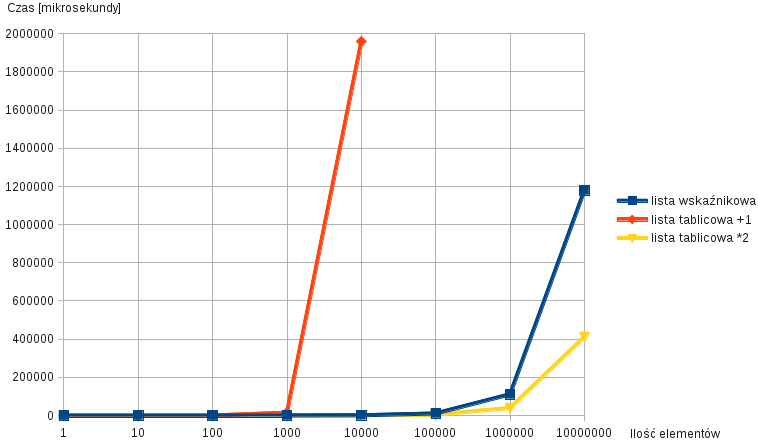
\includegraphics[scale=0.9]{wykres1}
 \caption{Wykres przedstawiający czas wczytywania elementów w programie}
\end{figure}

\pagebreak

\begin{figure}
 \centering
  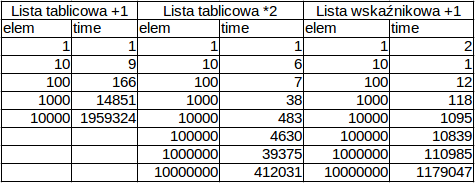
\includegraphics[scale=1]{tabela}
 \caption{Tabela z wartościami wypisanymi na wykresie}
\end{figure}
\end{landscape}

\end{document}
